\subsection{Height of Semilattice:}
\begin{itemize}
    \item \textbf{Definition}: It is defined as the largest number of greater than($>$) relations that would fit in a descending order.
    \par It can also be defined as the longest path length in the semilattice diagram.
    \item \textbf{Set of values $V$ and a partial order} For eg. in a semilattice with power set of $n$ definitions as the set of values $V$ and set intersection($\cap$) as the meet operator there would be 2\textsuperscript{n} number of elements but the height of the semilattice would be $n$ as that is the maximum path length in the graph(as can be seen in the figure \ref{fig:height_semilattice}). As we go down on each edge the cardinality reduces by 1 and the longest path is from complete set to null set of length $n$.
    \begin{figure}
    \centering
    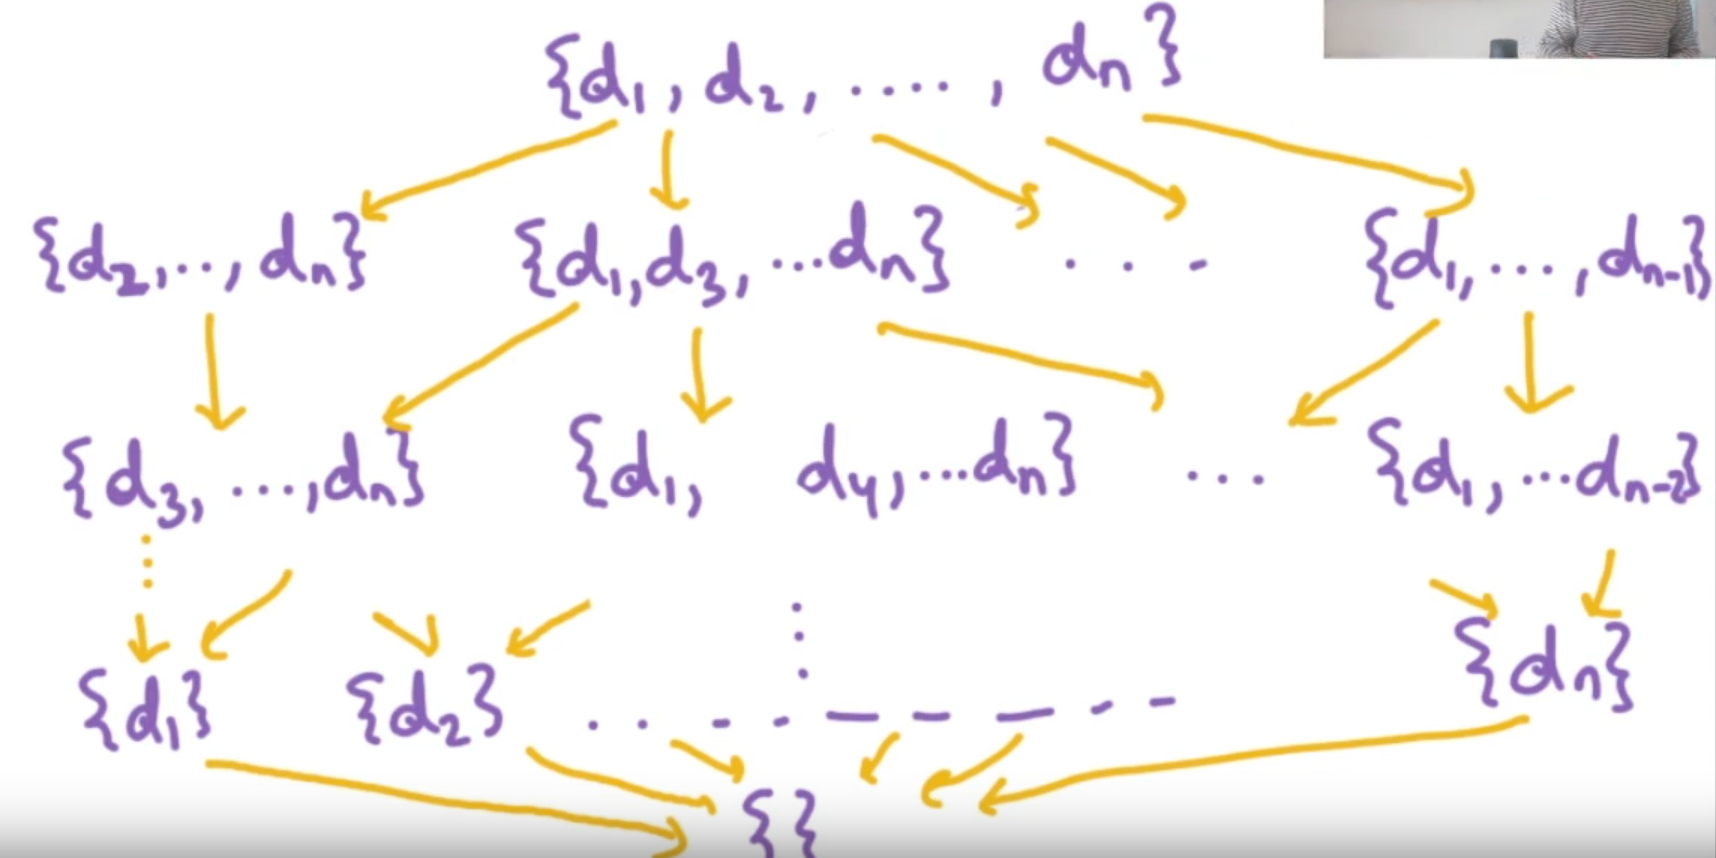
\includegraphics[width=1\linewidth]{images/semilattice_height.png}
    \caption{Semilattice height example}
    \label{fig:height_semilattice}
    \end{figure}
    \par Similarly, for DFA of reaching definitions the height of the semilattice is the number of definitions whereas the number of values is exponential in number of definitions.
    \item Now, There could be infinite height semilattices also having infinite no. of values(eg. set of integers with $max$ as the meet operator) but even with infinite no. of elements in the semilattice it’s height can still be finite, for eg. in case of constant propagation.
    \item Height of the semilattice is an important property because, one of the requirements for the fixed point iteration to converge is that the semilattice height is finite, if it’s infinite then the iteration is not guaranteed to converge.
\end{itemize}
